\documentclass[10pt,twocolumn]{article} 

% use the oxycomps style file
\usepackage{oxycomps}
\usepackage{graphicx}

% read references.bib for the bibtex data
\bibliography{references}

% include metadata in the generated pdf file
\pdfinfo{
    /Title (Tutorial report)
    /Author (Victor Zhu)
}

% set the title and author information
\title{Tutorial Report}
\author{Victor Zhu}
\affiliation{Occidental College}
\email{hzhu@oxy.edu}

\begin{document}

\maketitle


\section{Methodology}

\subsection{Set up and Basic Game Architecture}
In order to create the battleground for my players, First I have to create a canvas and start to add color to it. Then I put two images on each side with different colors. One is set to be the player area another is the enemy area. These two places are the place where players and the enemy place their cards. Then I created more UIimage as cards. I saved them as prefab and deleted them because they are not required for the moment. 
After finishing the basic background, I worked on the draw button.(as shown in figure 1) The draw button will “draw” the card. First, I created a button from the ui option of unity object, then I created a script to configure the draw button. The script define the button in two ways. One is how it will react when mouse click on it and how it will get cards and land it in the player’s space. Once that is done, then I coded a for loop to let the draw action happen 5 times to allow the player to draw all its deck.  
\begin{figure}[ht]
  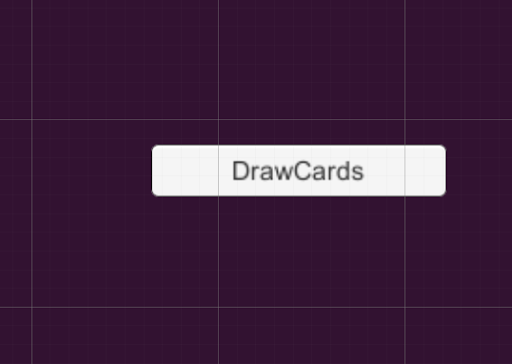
\includegraphics[width=\linewidth]{drawcardsbutton.png}
  \caption{Drawbutton.}
  \label{fig:Drawbutton}
\end{figure}
Then I configured the space between the cards to make my player area looks better. Then I do the same thing and allow the enemy to draw their cards. (as shown in figure 2)After draw function is finished, I worked on the “drag and drop” function of the game. I first start a new script call “draganddrop”. The drag and drop script is attached to the card and define how it will move. Then I add a box collider to card obejct to act more like physical card instead of a image.
\begin{figure}[ht]
  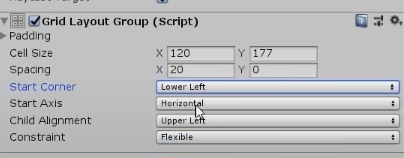
\includegraphics[width=\linewidth]{cardspacing.png}
  \caption{card spacing by changing spacing option }
  \label{fig:cardspacing}
\end{figure}
	After I define basic of card movement, I put another UI image into the middle the of battlefield. This image field will served as the battlezone for the player and player’s enemy. I am going to name this image field as the drop zone. Since I want all cards to be only be dropped into the dropzone, so I change some of method of  “draganddrop”script to make sure that cards can only be dropped into the dropzone or the player area and no where else. Then I added a method to define the collision between the other UI images and Card prefabs, so cards always come up on top
\subsection{Canvas Cleanup and Advanced Interactivity}
In this section, I am going to revised some of my code to create a better outlook and a better user experience.
I first try to change the drag and drop method in “draganddrop” script. I add in a method so that when the player drag the cards to the opposing area, ie ,player area to enemy  area  or vice versa, it will come back their own area.
After I finish that method, I create a new script call Cardzoom which allows the player to zoom in on cards when the player ‘s cursor hovers over the cards. After I have finished the script , I went to unity physic option to untangle the clide method, so my zoomed -in card will not collide with the other UIs.
\subsection{Multiplayer Basics with Mirror}
In this section, I will add simple multiplayer function to my game using mirror. First i imported mirror from the unity asset store. After importing the package, I created a empty game object and call it networkmanager.  In the inspector panel of the networkmanager, I add a component call network manager hud which will show the the networkmanager status when we start the game. It looks like figure 3. 

\begin{figure}[ht]
  \includegraphics[width=\linewidth]{networkmanagehud.png}
  \caption{Network Manager HUD}
  \label{fig:HUD}
\end{figure}

I then created an empty game object and called it the playermanager and add it to the player prefab in the network manager’s inspector panel. For now, I only have one client on this network which is my computer.  In order to play the game online simultaneously with another client, I have to build the game every time I run it. So I go to the file option in Unity and selected the build setting.  Through the build setting, I am able to build the game. 
	I create a new script called the player-manager and add it to the playermanager object. This script first adds the cards to both of the player’s hand when the game instance starts. Then I set a method that limits the player to play only their own cards. 
As of now, a basic version of the game is finally finished
\section{Evaluation Metrics}
The main Evaluation Metric of this project is the user experience. As I run the project and play it, there is nothing very impressive about the game, since there is only a basic framework the game. However, I do see the potential of the framework as it can support the multiplayer game. 
\section{Results and Discussion}
As I have finished this tutorial, I have created a framework for a simple multiplayer 2d card game. There are many things lacking in this basic framework, such as the health, cost of playing a card, and card effect system. All of these are essential to the game because it determines who will win. A proper health system is vital to a multiplayer card game. Take Hearthstone, for example, the game can be won only if one of the player’s health has reduced below zero. The health system gives players a purpose during the game. The cost of playing a card is also very important because it gives the meaning of the card and makes the player strategize their move. The card effect system is going to make cards more unique and add more interesting gameplay to the game.  I have done this prototype of the game in unity  2019 2.15f1, many of its features are not supported in the current version of unity and C-sharp code. It did cost me a lot of problems when I was coding the project. Sometimes I have to go to another tutorial online to finish some of the features in Mr. Fazan’s tutorial. Luckily enough, Mr. Fazan also offers the 2021 version of the project, I find myself consulting that tutorial many times as well. In order to build on this prototype for my upcoming project, I will have to add a proper health system, a cost of cards system, and a card effect system. My game is planned to be in the sci-fi RPG genre, all these systems are important because they will help the player to be immersed in the game. The health system would make players worry about the survival of the character. The cost of the card system will make players think about their strategy and also help me, the developer, to balance the cards. The effect of the cards is also essential because my game will be a role-playing card game. All the cards have to represent a part of the action of the player’s avatar in the game such as an attack, block, or even burn, freeze and poisons, etc.    




\end{document}
